\subsection{Résultats}
Nous allons ici présenter les résultats obtenus en expérimentant les algorithmes de Toussaint et de Ritter avec 1663 instances de test de la base VAROUMAS fournis. Les algorithmes ont été exécutés sur un ordinateur équipé de 12GB RAM et d'un processeur \textit{Intel Core i7 4790K} cadencé à 4.00GHz tournant sous \textit{Windows 10 Pro 64-bit}.

\begin{center}
\begin{tabular}{|*{4}{c|}}
    \hline
       & Graham  & Toussaint  & Ritter \\
    \hline
     Temps min.  & 0.025103 ms  &0.25538 ms  & 0.009989 ms \\
    \hline
     Temps moy.  & 0.039666 ms  & 0.306384 ms  & 0.019886 ms \\
    \hline
     Temps max.  & 1.697752 ms  & 6.256938 ms & 1.028693 ms \\
    \hline
\end{tabular}
\captionof{table}{Temps d'exécution}
\label{texec}
\end{center}

\begin{figure}[ht]
\begin{center}
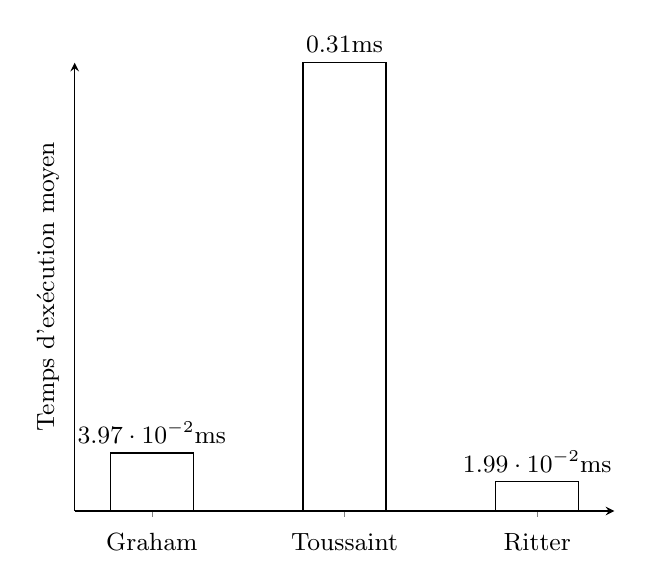
\begin{tikzpicture}[font=\small]
    \begin{axis}[
      ybar,
      bar width=30pt,
      ylabel={Temps d'exécution moyen},
      ymin=0,
      ytick=\empty,
      xtick=data,
      axis x line=bottom,
      axis y line=left,
      enlarge x limits=0.2,
      symbolic x coords={Graham, Toussaint,Ritter},
      xticklabel style={anchor=base,yshift=-\baselineskip},
      nodes near coords={\pgfmathprintnumber\pgfplotspointmeta ms}
    ]
      \addplot[fill=white] coordinates {
      	(Graham,0.039666)
        (Toussaint,0.306384)
        (Ritter,0.019886)
      };
    \end{axis}
\end{tikzpicture}
\label{gtime}
\end{center}
\end{figure}

\begin{center}
\begin{tabular}{|*{3}{c|}}
    \hline
       & Toussaint  & Ritter \\
    \hline
     Efficacité  & 25,23\%  & 20,52\%  \\
    \hline
\end{tabular}
\captionof{table}{Efficacité}
\label{eff}
\end{center}

\begin{figure}[ht]
\begin{center}
\begin{tikzpicture}[font=\small]
    \begin{axis}[
      ybar,
      bar width=30pt,
      ylabel={Efficacité},
      ymin=0,
      ytick=\empty,
      xtick=data,
      axis x line=bottom,
      axis y line=left,
      enlarge x limits=0.2,
      symbolic x coords={Toussaint,Ritter},
      xticklabel style={anchor=base,yshift=-\baselineskip},
      nodes near coords={\pgfmathprintnumber\pgfplotspointmeta\%}
    ]
      \addplot[fill=white] coordinates {
        (Toussaint,25.23)
        (Ritter,20.52)
      };
    \end{axis}
\end{tikzpicture}
\label{geff}
\end{center}
\end{figure}